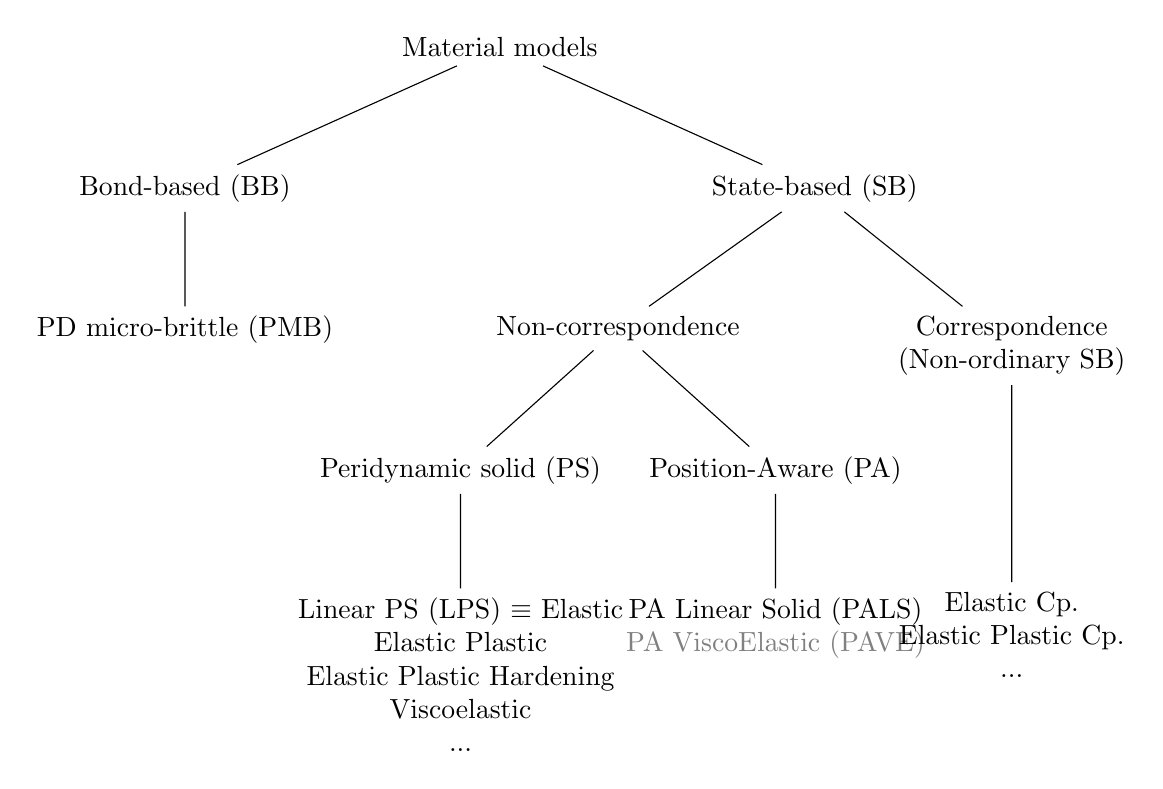
\begin{tikzpicture}[
% for small:
% for footnotesize:
  basic/.style = {anchor=north},
  level distance=1.5cm,
  level 1/.style={basic,sibling distance=8cm},
  %level 2/.style={basic,sibling distance=6cm},
  level 2/.style={basic,sibling distance=5cm},
  %level 3/.style={basic,sibling distance=5.0cm},
  level 3/.style={basic,sibling distance=4.0cm},
  level 4/.style={basic,sibling distance=1.75cm},
  level 5/.style={basic,sibling distance=1.0cm},
  %growth parent anchor = north,
]
  \node {Material models}
    child {node {Bond-based (BB)}
      %child {node {Peridynamic micro-brittle (PMB)}}
      child {node {PD micro-brittle (PMB)}}
    }
    child {node {State-based (SB)}
      child {node {Non-correspondence}
        child {node {Peridynamic solid (PS)}
          child {node[align=center] {%
            Linear PS (LPS) $\equiv$ Elastic\\%
            Elastic Plastic\\%
            Elastic Plastic Hardening\\%
            Viscoelastic\\%
            ...%
          }}
        }
        child {node {Position-Aware (PA)}
          child {node[align=center] {%
            %Position-Aware Linear Solid (PALS)\\%
            %\textcolor{gray}{Position-Aware ViscoElastic (PAVE)}%
            PA Linear Solid (PALS)\\%
            \textcolor{gray}{PA ViscoElastic (PAVE)}%
          }}
        }
      }
      child {node[align=center] {Correspondence\\(Non-ordinary SB)}
        child {%node {}
          child {node[align=center] {%
            Elastic Cp.\\%
            Elastic Plastic Cp.\\%
            ...%
          }}
        }
      }
    };
\end{tikzpicture}